%=======================================================================
\section{Introduction}
\label{sec_pfoobar_intro}

An introduction to the MOOS app should concisely convey what the app does, 
similar to the short synopsis output when the user types --help on the 
command line. If it is similar to another MOOS app, it may be good to 
state up front how it is different and why this app was written rather
than just using the old one. A bulleted list of functionality may also
be appropriate, e.g., pFooBar primarily does:

\begin{packed_itemize}

\item Subcribes for FOO.

\item Converts it to BAR.

\item Publishes it as BAR.

\end{packed_itemize}
\vspace{0.05in}

Sometimes a figure describing the workings of the app may be just the thing
to get the big picture across, as in Figure \ref{big_picture}

\begin{figure}[H]
  \begin{minipage}[b]{0.99\textwidth}
    \centering 
    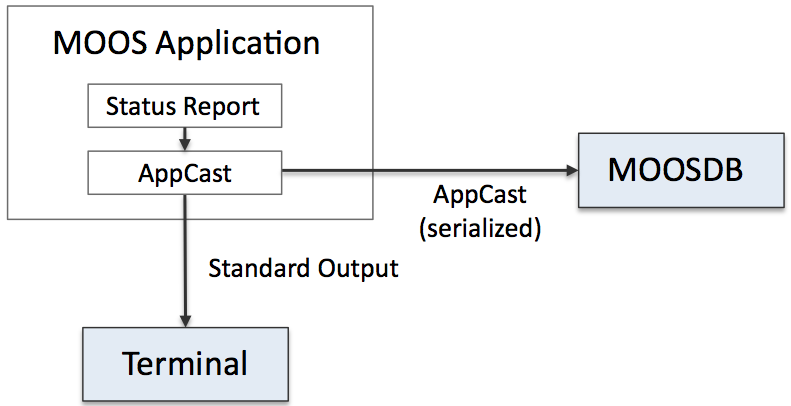
\includegraphics[width=0.5\textwidth]{figures/moos_withappcast.png}
  \end{minipage}
  \caption{An appcasting MOOS app produces terminal by repeatedly
    generating and sending an {\em appcast} to the terminal. The
    appcast is a also serialized and published to the MOOSDB for other
    MOOS applications to consume.}
\label{big_picture}
\end{figure}
\vspace{0.05in}

